\documentclass[11pt]{article}

\usepackage[slovene]{babel}
\usepackage[T1]{fontenc}
\usepackage[utf8]{inputenc}
\usepackage{lmodern}

\usepackage{amssymb}
\usepackage{amsmath}
\usepackage{amsthm}

\usepackage{enumerate}
\usepackage{graphicx}

\usepackage[parfill]{parskip}

\theoremstyle{definition} % tekst napisan pokoncno
\newtheorem{definicija}{Definicija}[section]
\newtheorem{primer}[definicija]{Primer}
\newtheorem{opomba}[definicija]{Opomba}

\theoremstyle{plain} % tekst napisan posevno
\newtheorem{lema}[definicija]{Lema}
\newtheorem{izrek}[definicija]{Izrek}
\newtheorem{trditev}[definicija]{Trditev}
\newtheorem{posledica}[definicija]{Posledica}

\newcommand{\R}{\mathbb R}
\newcommand{\N}{\mathbb N}
\newcommand{\Z}{\mathbb Z}
\newcommand{\C}{\mathbb C}
\newcommand{\Q}{\mathbb Q}

\DeclareMathOperator {\stopnja} {deg}

\title{Problem londonskega stolpa}
\author{Ines Meršak}
\date{16.~11.~2015}

\begin{document}
\maketitle

%\begin{frame}
%    Kratka predstavitev:
%    \begin{itemize}
%        \item klasičen problem londonskega stolpa - opis igre
%        \item osnovne definicije teorije grafov
%        \item klasičen problem londonskega stolpa - lastnosti grafa (Hamiltonova pot, etc.)
%        \item posplošen londonski stolp - definicija, povezanost, planarnost
%        \item primeri uporabe v psihologiji
%    \end{itemize}
%\end{frame}

\section{Klasični problem londonskega stolpa}
Ta problem je izumil Tim Shallice, profesor nevropshilogije, leta 1982 -- od takrat dalje se londonski stolp pogosto uporablja v psihologiji za preučevanje stanja bolnikov.

Problem je sledeči:
\begin{itemize}
    \item imamo 3 enako velike krogle različnih barv (recimo modra, rdeča, rumena)
    \item poleg tega imamo 3 palice različnih velikosti; na prvo lahko postavimo samo eno kroglo, na drugo dve, na tretjo tri
    \item cilj igre je priti iz trenutnega stanja v neko dano stanje z minimalnim številom potez
    \item najboljši način za vizualizacijo tega problema je s pomočjo grafa - zato si najprej poglejmo nekaj osnovnih definicij
\end{itemize}

\subsection{Osnovne definicije teorije grafov}
\begin{itemize}
    \item graf $ G = (V, E) $ je urejen par, kjer je $V$ množica vozlišč grafa in $E$ množica neurejenih parov vozlišč (te elemente imenujemo povezave); vozlišča predstavimo kot točke v ravnini, povezave pa kot krivulje med njimi
    \item $u$ in $v$ sta \emph{sosednji vozlišči}, če obstaja povezava med njima
    \item \emph{soseščina} vozlišča $u$ je $N(u) = \{x \in V;\ ux \in E\}$
    \item \emph{stopnja} vozlišča $u$: $\stopnja u  = \lvert N(u) \rvert$ je število sosedov tega vozlišča
    \item \emph{sprehod} v grafu je zaporedje vozlišč $v_1,\ldots v_k$, da za vsak $i$ velja $v_i v_{i+1} \in E$
    \item graf je \emph{povezan}, če za poljuben par vozlišč obstaja sprehod med njima
    \item \emph{premer} grafa je največja minimalna razdalja med pari vozlišč; če vzamemo poljubno vozlišče v grafu, potem lahko pridemo do drugega poljubnega vozlišča preko $d$ ali manj povezav, kjer je $d$ premer grafa
    \item \emph{ravninski} graf je graf, ki ga lahko narišemo v ravnini brez križanja povezav
    \item pot v grafu, ki vsebuje vsa vozlišča, je \emph{Hamiltonova pot}
\end{itemize}


\subsection{Graf klasičnega problema londonskega stolpa}
Označimo krogle s številkami 1, 2, 3, pri čemer je npr.\ krogla 1 modra, krogla 2 rdeča, krogla 3 pa rumena. Začetek naslednje palice bomo nakazali z |, krogle pa bomo naštevali od vrha proti dnu palice.
Na primer: stanja na prejšnji sliki so |3|12 in |21|3.
Vidimo, da je minimalno število potez pri tem primeru 4 in da obstaja samo eno najkrajše zaporedje potez.
\begin{figure}[h]
    \centering
    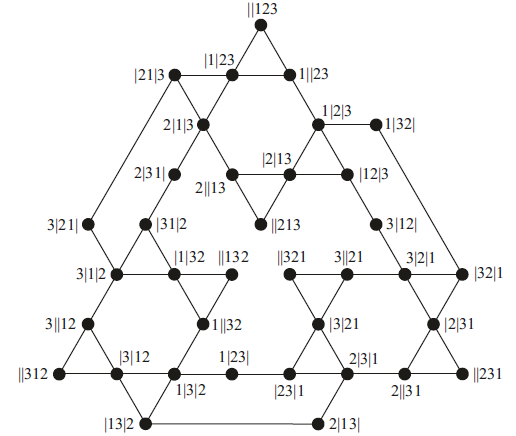
\includegraphics[height=200pt]{img/tolgraph.png}
\end{figure}

\subsubsection{Lastnosti grafa}
\begin{itemize}
    \item 36 vozlišč (36 možnih stanj)
    \item utežene stopnje vozlišč (12 vozlišč stopnje 2, 3, 4)
    \item premer grafa je 8
    \item ravninski (narisan je v ravnini, povezave se nikjer ne križajo)
    \item vsebuje Hamiltonovo pot
\end{itemize}


\section{Posplošen londonski stolp}
Graf klasičnega problema je majhen, možnih stanj je malo, zato je za testiranje odraslih ljudi naloga včasih prelahka; Jenny R.\ Tunstall je prva predlagala razširitev na 4 krogle s podaljšanimi palicami (vsaka je podaljšana za eno enoto).

Poglejmo si posplošitev tega problema na $p$ palic in $n$ krogel različne barve, pri čemer je $p \geq 3 \text{ in } n \geq 2$. Vsako palico označimo s številom $k \in [p]$, pri čemer je $h_k$ višina palice (ta predstavlja število krogel, ki jih drži palica). Krogle označimo z 1 do $n$ -- te lahko razporejamo na palice. Veljati mora $n \leq \sum_{k=1}^p h_k$. Poteza je veljavna, če vrhnjo kroglo neke palice prestavimo na vrh druge, pod pogojem, da je na tej palici manj kot $h_k$ krogel.

Vsako stanje krogel lahko enolično predstavimo s permutacijo $s \in S_{n+p}$, $S$ je simetrijska grupa. Pri tem je $s_i$ položaj krogle $i$, če $i \in [n] $, ali dna palice $i-n$, če je $i \in [n+p] \setminus [n] $. Položaje beremo od vrha palice proti dnu in z leve proti desni za palice (kot pri klasičnem problemu).
Naš primer: $s = 452136$.
{\small $s$ bomo zapisali v obliki $ \sum_1 | \ldots | \sum_p $, kjer je $\sum_k$ niz oznak krogel v položajih od $s_{n+k-1} + 1$ do $s_{n+k}-1$ od vrha palice navzdol. $s_{n+0} = 0$ in ne $s_n$. Vertikalne pipe spet označujejo začetek dna palice.}

\begin{definicija}
    \emph{Londonski graf} $L_h^n$, kjer je $p \geq 3,\ n \geq 2,\ h \in [n]^p,\  \sum_{k=1}^p h_k \geq n$:
    \begin{itemize}
        \item vozlišča: vse permutacije $s \in S_{n+p}$, za katere velja:
        \[\forall k \in [p]:\ 1 \leq s_{n+k} - s_{n+k-1} \leq h_k + 1,\ s_{n+p} = n + p ,\]
        \item povezave: vsaki dve stanji (oz.\ pripadajoči permutaciji), med katerima lahko prehajamo z veljavno potezo, sta povezani
    \end{itemize}
\end{definicija}

BŠS $h_1 \leq h_2 \leq \ldots \leq h_p$.

Dve lastnosti, pomembni za uporabo londonskega stolpa v psihologiji, sta povezanost in ali je graf ravninski.
Povezanost zato, da je problem rešljiv, ne glede na to, katero začetno in končno stanje si izmislimo.

Potreben pogoj za povezanost Londonskega grafa je 
\[ n \leq \sum_{k=1}^{p-1} h_k. \]
Namreč, možna mora biti razporeditev krogel, kjer najdaljša palica ostane prazna. Če so ostale palice zapolnjene, s tiste palice ne moremo več premakniti nobene krogle. 

To je lep primer potrebnega pogoja, ki je tudi zadosten.
\begin{izrek}
Londonski graf $L_h^n$ je povezan natanko tedaj, ko velja pogoj
\[ n \leq \sum_{k=1}^{p-1} h_k. \]
\end{izrek}


\section{Uporaba}
\begin{itemize}
    \item Problem londonskega stolpa je bil razvit z namenom merjenja sposobnosti načrtovanja in reševanja problemov pri bolnikih s poškodbami čelnega režnja možganov.
    \item Slabo reševanje londonskega stolpa se interpretira kot nezmožnost učinkovitega načrtovanja.
    \item Uporabljen za ocenjevanje napredka bolezni pri bolnikih z Alzheimerjevo in Parkinsonovo boleznijo.
    \item Uporabljen za opazovanje vedenja majhnih otrok pri reševanju problemov.
\end{itemize}

\end{document}
